%%%%%%%%%%%%%%%%%%%%%%%%%%%%%%%%%%%%%%%%%
% University/School Laboratory Report
% LaTeX Template
% Version 3.1 (25/3/14)
%
% This template has been downloaded from:
% http://www.LaTeXTemplates.com
%
% Original author:
% Linux and Unix Users Group at Virginia Tech Wiki 
% (https://vtluug.org/wiki/Example_LaTeX_chem_lab_report)
%
% License:
% CC BY-NC-SA 3.0 (http://creativecommons.org/licenses/by-nc-sa/3.0/)
%
%%%%%%%%%%%%%%%%%%%%%%%%%%%%%%%%%%%%%%%%%

%----------------------------------------------------------------------------------------
%	PACKAGES AND DOCUMENT CONFIGURATIONS
%----------------------------------------------------------------------------------------

\documentclass{article}

\usepackage{graphicx} % Required for the inclusion of images
\usepackage{natbib} % Required to change bibliography style to APA
\usepackage{amsmath} % Required for some math elements 
\usepackage{amsthm}
\usepackage[hyphens]{url}
\usepackage{hyperref}
\usepackage{subcaption}
\usepackage{float}
\usepackage{array}
\usepackage{amssymb}
\usepackage{calrsfs}
\usepackage{pgfplots}
\pgfplotsset{width=10cm,compat=1.9}
\usepackage{bytefield}


\setlength\parindent{0pt} % Removes all indentation from paragraphs

\newtheorem*{remark}{Theorem}
\newtheorem*{definition}{Definition}

%----------------------------------------------------------------------------------------
%	DOCUMENT INFORMATION
%----------------------------------------------------------------------------------------

\title{Homework \#4 \\Elliptic Curves \\[0.2em]\small{}CNS Course Sapienza} % Title and subtitle

\author{Riccardo \textsc{Prinzivalle}, 1904064} % Author name

\date{November 20, 2020} % Date for the report

\begin{document}

\maketitle % Insert the title, author and date

%----------------------------------------------------------------------------------------
%	SECTION 0
%----------------------------------------------------------------------------------------

\section{Homework Goal}

This homework contains a basic introduction on Elliptic Curves (EC), the general idea on the math basis, the Discrete Logarithm Problem with EC and the practical utilize of EC in cryptography. All this work is mainly based on YouTube lesson held by Professor Paar \cite{video1}, \cite{video2} and on his introductory book to cryptography \cite{10.5555/1721909}.

%----------------------------------------------------------------------------------------
%	SECTION 1
%----------------------------------------------------------------------------------------

\section{Elliptic Curves Motivation}

Elliptic Curves are the main trend in asymmetric encryption today: why is their usage so spread? This question has a simple answer: it is sufficient to look at table \ref{tab:keyLen}, where there is a comparison of the key length needed to guarantee the same level of security. 
 
\renewcommand{\arraystretch}{2}

\begin{table}[H]
	\begin{center}
		\begin{tabular}{ |c || c | c | c | c | c | c | }
			\hline
			Algorithm Family & Cryptosystems & \multicolumn{4}{c |}{Security Level (bit)}\\
			& & 80 & 128 & 192 & 256\\ [0.5ex] 
			\hline\hline
			Integer Factorization & RSA & 1024 & 3072 & 7680 & 15360  \\ 
			
			Discrete Logarithm & DH, DSA, Elgamal & 1024 & 3072 & 7680 & 15360  \\ 
			
			Elliptic Curves & ECDH, ECDSA & 160 & 256 & 384 & 512  \\ 
			\hline
			Symmetric key & AES, 3DES &  80 & 128 & 192 & 256  \\ 
			\hline
		\end{tabular}
		\caption{Key length comparison in public key and symmetric key algorithm}
		\label{tab:keyLen}
	\end{center}
\end{table}

The bare minimum number of bits is defined by the symmetric key encryption scheme, we cannot have a smaller key with respect to the symmetric case and have the same level of security; then asymmetric schemes need, in general, a large number of bits to guarantee the same level of security, the fact is that elliptic curves cryptography needs less than $\cfrac{1}{10}$ of the bits needed for another asymmetric scheme supposed the same level of security, and this relationship become smaller as the level of security grows. Indeed, if one wants to use a public key cryptography scheme, elliptic curves are the suggested choice to guarantee security without using much computational effort.

%----------------------------------------------------------------------------------------
%	SECTION 3
%----------------------------------------------------------------------------------------

\section{Mathematical background}

The base idea besides elliptic curves lies on common calculus background: everyone knows the circumference equation, isn't it? It is $x^2 + y^2 = r^2$, but what if we add coefficients in front of the variables? We end up with an ellipse: $ax^2 + by^2 = r^2$, whose graph can be seen in Fig. \ref{fig:ellipse}. 

\begin{figure}[H]
	\centering
	\begin{subfigure}{.49\textwidth}
		\centering
		\begin{tikzpicture}
			\begin{axis}[
				xmin=-4,
				xmax=4,
				ymin=-6.6,
				ymax=7,
				xlabel={$x$},
				ylabel={$y$},
				scale only axis,
				axis lines=middle,
				domain=-4:4,      
				samples=1000,
				smooth,
				% use same unit vectors on the axis
				axis equal image=true,
				legend pos=south east,
				]
				\addplot [red] {sqrt(-0.2*x^2+2)};
				\addlegendentry{$y^2=-0.2x^2+2$};
				\addplot [red] {-sqrt(-0.2*x^2+2)};
			\end{axis}
		\end{tikzpicture}
		\caption{Ellipse}
		\label{fig:ellipse}
	\end{subfigure}
	\begin{subfigure}{.49\textwidth}
		\begin{tikzpicture}
			\begin{axis}[
				xmin=-4,
				xmax=4,
				ymin=-6.6,
				ymax=7,
				xlabel={$x$},
				ylabel={$y$},
				scale only axis,
				axis lines=middle,
				domain=-4:3,      
				samples=300,
				smooth,
				% use same unit vectors on the axis
				axis equal image=true,
				legend pos=south east,
				]
				\addplot [red] {sqrt(x^3-3*x+3)};
				\addlegendentry{$y^2=x^3-3x+3$};
				\addplot [red] {-sqrt(x^3-3*x+3)};
				\addplot [mark=none, domain=3:4, red, dashed] {sqrt(x^3-3*x+3)};
				\addplot [mark=none, domain=3:4, red, dashed] {-sqrt(x^3-3*x+3)};
			\end{axis}
		\end{tikzpicture}
		\centering
		\caption{Elliptic Curve}	
		\label{fig:EC}
	\end{subfigure}
	\caption{Graphical comparison of ellipse and elliptic curve}
	\label{fig:graph}
\end{figure}
 
 Well, an elliptic curve is something much similar: the general equation is $y^2 = x^3 + ax + b$, and an example of it can be seen in Fig. \ref{fig:EC}. We can easily see from the plot that this family of curves has symmetry with respect to $x$ axis. \newline
 In order to perform cryptography with elliptic curves, we need to reduce their usage to a special family of them: instead of defining them over the real domain $\mathbb{R}$, we use the integer group $\mathbb{Z}_{p}$ (which is a set of integer numbers with a group operator and is closed w.r.t. this operation), with $p > 3$. In addition, the elliptic curve equation is reduced in$\mod p$, and the coefficients must satisfy the following equation to remove curves that are useless or too easy to break: $4a^3 + 27b^2 \ne{0}$. To fulfill the group operation, we need to add an imaginary point at infinity, $\mathcal{O}$. \newline
 Now that we have defined the elliptic curves of interest, we need to define a group over them, which is the basis of cryptography: in order to accomplish this task, we need a set of elements, which are the points belonging to the elliptic curves, and then we need a group operator to fulfill the group law. It is possible to have both a geometrical and analytical interpretation of this operator; here we start with the geometrical one since it is easier to understand and more explicative.
 The geometric interpretation starts by drawing the elliptic curve without modulo reduction and defined on $\mathbb{R}$, so we can easily visualize the curve in a 2D graph as those in Fig. \ref{fig:groupOp}. The group operation can be divided into 2 simpler case: the addition of two different point and the addition of the same point, called also \textit{doubling}. 
 
 \begin{figure}[H]
 	\centering
 	\begin{subfigure}{.49\textwidth}
 		\centering
 		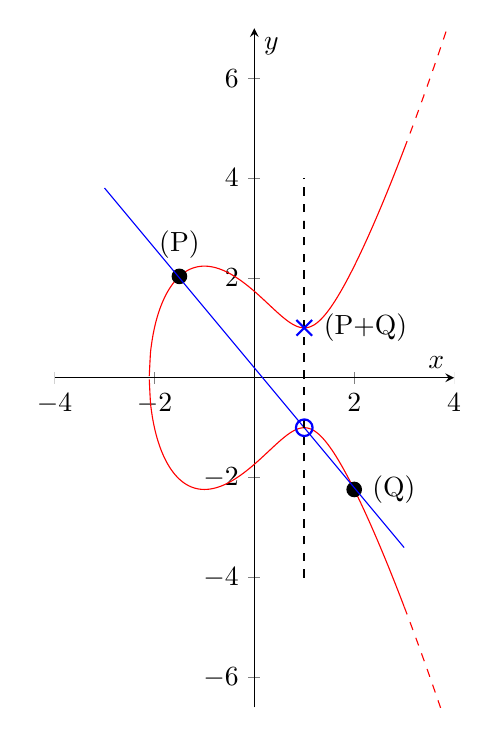
\begin{tikzpicture}[]
 			\begin{axis}[
 				xmin=-4,
 				xmax=4,
 				ymin=-6.6,
 				ymax=7,
 				xlabel={$x$},
 				ylabel={$y$},
 				scale only axis,
 				axis lines=middle,
 				domain=-4:3,      
 				samples=300,
 				smooth,
 				% use same unit vectors on the axis
 				axis equal image=true,
 				legend pos=south east,
 				]
 				\addplot [red] {sqrt(x^3-3*x+3)};
 				\addplot [red] {-sqrt(x^3-3*x+3)};
 				\addplot [mark=none, domain=3:4, red, dashed] {sqrt(x^3-3*x+3)};
 				\addplot [mark=none, domain=3:4, red, dashed] {-sqrt(x^3-3*x+3)};
 				\node[label={90:{(P)}},circle,fill,inner sep=2pt] at (axis cs:-1.5,{sqrt(4.125)}) {};
 				\node[label={0:{(Q)}},circle,fill,inner sep=2pt] at (axis cs:2,{-sqrt(5)}) {};
 				\addplot [blue, domain=-3:3] {-1.2*x+0.2};
 				\addplot [only marks,mark=o,color=blue,mark size=3, thick] coordinates { (1,{-sqrt(1)})};
 				\addplot[thick, samples=50, smooth, dashed] coordinates {(1,-4)(1,4)};
 				\addplot [only marks,mark=x,color=blue,mark size=4, thick] coordinates { (1,{sqrt(1)})};
 				\node[label={0:{(P+Q)}}] at (axis cs:1,{sqrt(1)}) {};
 			\end{axis}
 		\end{tikzpicture}
 		\caption{Point addition}
 		\label{fig:addition}
 	\end{subfigure}
 	\begin{subfigure}{.49\textwidth}
 		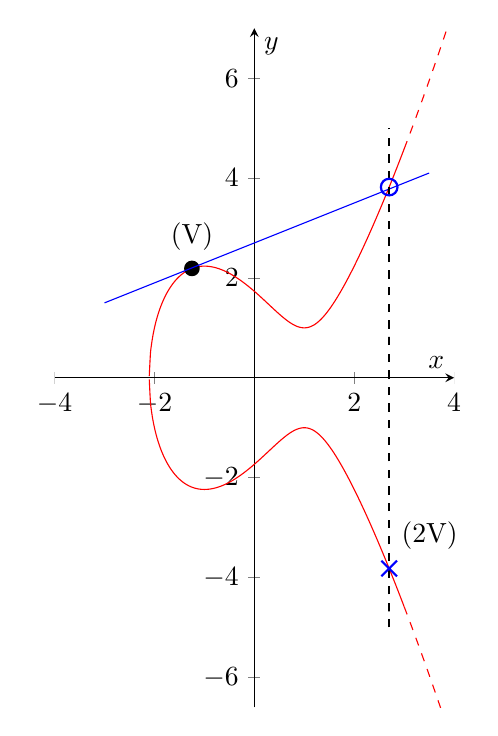
\begin{tikzpicture}
 			\begin{axis}[
 				xmin=-4,
 				xmax=4,
 				ymin=-6.6,
 				ymax=7,
 				xlabel={$x$},
 				ylabel={$y$},
 				scale only axis,
 				axis lines=middle,
 				domain=-4:3,      
 				samples=300,
 				smooth,
 				% use same unit vectors on the axis
 				axis equal image=true,
 				legend pos=south east,
 				]
 				\addplot [red] {sqrt(x^3-3*x+3)};
 				\addplot [red] {-sqrt(x^3-3*x+3)};
 				\addplot [mark=none, domain=3:4, red, dashed] {sqrt(x^3-3*x+3)};
 				\addplot [mark=none, domain=3:4, red, dashed] {-sqrt(x^3-3*x+3)};
 				\node[label={90:{(V)}},circle,fill,inner sep=2pt] at (axis cs:-1.25,{sqrt(4.796875)}) {};
 				\addplot [blue, domain=-3:3.5] {0.4*x+2.7};
 				\addplot [only marks,mark=o,color=blue,mark size=3, thick] coordinates { (2.7,{sqrt(14.583)})};
 				\addplot[thick, samples=50, smooth, dashed] coordinates {(2.7,-5)(2.7,5)};
 				\addplot [only marks,mark=x,color=blue,mark size=4, thick] coordinates { (2.7,{-sqrt(14.583)})};
 				\node[label={75:{(2V)}}] at (axis cs:2.7,{-sqrt(14.583)}) {};
 			\end{axis}
 		\end{tikzpicture}
 		\centering
 		\caption{Point doubling}	
 		\label{fig:doubling}
 	\end{subfigure}
 	\caption{Graphical interpretation of group operator}
 	\label{fig:groupOp}
 \end{figure}

The first situation is represented in Fig. \ref{fig:addition}: we want to sum points P and Q, we draw the secant line passing through this two points, then, due to the particular form of the elliptic curve, we are able to find a new intersection between the EC and the secant other than the two point to be summed, this new point is highlighted by a circle in the figure, finally this point is mirrored w.r.t. the x axis and the resulting point is the sum between P and Q, and it is denoted by an \textbf{x} in the plot.\newline
In the other case, we need to develop something different: since we are adding the same point, we cannot define a secant line, but, if we think at point Q of Fig. \ref{fig:addition} and we try to move it along the EC towards V, we easily see that the secant becomes the tangent to the EC in point V as in Fig. \ref{fig:doubling}. Given this mind set, it is easy to apply the same reasoning as in the previous case: we seek for the intersection between the tangent line and the EC, then project this point mirroring it w.r.t. the x axis and we end up with the point 2V. All this is represented in Fig. \ref{fig:doubling}. \newline
The geometrical interpretation is fine to visualize the reasoning and the idea, but what if we want to use this mind set in practice? We need to develop an analytical formulation: take the idea in the case of addition, then with doubling it's similar. We start from the EC equation $EC: y^2 = x^3 + ax +b$ and we define the secant passing through points P and Q as $\mathcal{L}: y = sx + m$, whose coefficient can be easily found once we have the values of the two points to be added. We want to find the point to be mirrored, so we solve the system between $EC$ and $\mathcal{L}$, which simply is $s^2x^2 + m^2 + 2smx =  x^3 + ax +b$, whose only unknown is the variable $x$ (the other parameters are determined once we have the practical problem). This system admits 3 different solution: two of them are the points to be added and the third one is the mirror of the resulting point of the addition. With some computations, we end up with the addition formula:

\begin{equation}
	s = \cfrac{y_2 - y_1}{x_2 - x_1} \mod p
	\label{mat:addition}
\end{equation}

Equation \ref{mat:addition} gives us the slope of the secant line. A little extension to this formula: in implementation we use $(y_2 - y_1)(x_2 - x_1)^{-1} \mod p$ since inversion is easier to compute than division (multiplicative inverse can be computed by means of Extended Euclidean Algorithm). Similar reasoning and computation drive us to the formula of the slope in the case of doubling:

\begin{equation}
	s = \cfrac{3x_1^{2} + a}{2y_1} \mod p
\end{equation}

Now we are finishing our journey, but we still need one more thing: to define a group, it is necessary to have a neutral element for the group operator; something such that $P + ? = P$. If we understood correctly the addition mechanism, to end in P, we need to obtain a secant whose third intersection point with the EC is the mirror of P w.r.t. the x axis: so we need a vertical secant line, which is obtainable only by using an artificial point defined before as $\mathcal{O}$. This point is not a real point, we just created it to be at $+\infty$ or at $-\infty$ on y axis in order to obtain a vertical secant line. This behavior can be seen in Fig. \ref{fig:neutral}.

\begin{figure}[H]
	\centering
	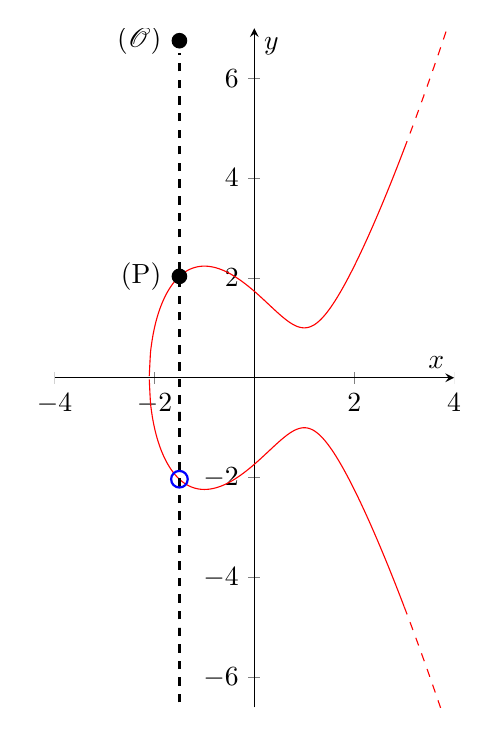
\begin{tikzpicture}[]
		\begin{axis}[
			xmin=-4,
			xmax=4,
			ymin=-6.6,
			ymax=7,
			xlabel={$x$},
			ylabel={$y$},
			scale only axis,
			axis lines=middle,
			domain=-4:3,      
			samples=300,
			smooth,
			% use same unit vectors on the axis
			axis equal image=true,
			legend pos=south east,
			]
			\addplot [red] {sqrt(x^3-3*x+3)};
			\addplot [red] {-sqrt(x^3-3*x+3)};
			\addplot [mark=none, domain=3:4, red, dashed] {sqrt(x^3-3*x+3)};
			\addplot [mark=none, domain=3:4, red, dashed] {-sqrt(x^3-3*x+3)};
			\node[label={180:{(P)}},circle,fill,inner sep=2pt] at (axis cs:-1.5,{sqrt(4.125)}) {};
			\node[label={180:{($\mathcal{O}$)}},circle,fill,inner sep=2pt] at (axis cs:-1.5,6.75) {};
			\addplot [only marks,mark=o,color=blue,mark size=3, thick] coordinates { (-1.5,-{sqrt(4.125)})};
			\addplot[thick, samples=50, smooth, dashed] coordinates {(-1.5,-6.5)(-1.5,6.5)};
		\end{axis}
	\end{tikzpicture}
	\caption{Group operator neutral element}
	\label{fig:neutral}
\end{figure}

The introduction of $\mathcal{O}$ allows to fulfill two different group properties:

\begin{itemize}
	\item $P + \mathcal{O} = P \hspace{1em} \forall P \in EC$
	\item $P + (-P) = \mathcal{O}  \hspace{1em} \forall P \in EC$
\end{itemize}

The second property needs some more explanation: $-P$ is the mirror of the point $P$ w.r.t. the x axis, so $-P = (x_p, -y_p)$, where the minus in front of $P$ comes from the group operator, while the minus in front of $y_p$ is the typical minus operation used in $\mathbb{R}$. With these properties the mathematical background comes to an end, we must only add a theorem without proof, which is the following:

\begin{remark}
	The points on an $EC$, including $\mathcal{O}$, have a cyclic subgroup. Under certain conditions, all points on an $EC$ form a cyclic group.
\end{remark} 

This theorem comes in handy when dealing with cryptography, since we need a cyclic subgroup to guarantee that a computation is easy to do in one way but hard to reverse. A cyclic subgroup is such that, if we apply repeatedly the group operation to a generator of the group, we will end up with generator itself after some number of iteration depending on the nature of the cyclic group.

%----------------------------------------------------------------------------------------
%	SECTION 4
%----------------------------------------------------------------------------------------

\section{Discrete Logarithm Problem with EC}

Once we have a cyclic group, it is useful to use it for the Discrete Logarithm Problem (DLP). This idea is also suggested by the previous analysis of tab. \ref{tab:keyLen}.\newline
We can synthesize the DLP problem on elliptic curve with the following definition:

\begin{definition}
	Given an elliptic curve E, if we consider a generator P of the cyclic subgroup derived from E and another element T, the discrete logarithm problem is finding the integer d, where 1 $\leq$ d $\leq$ \#E (where \#E is the cardinality of the cyclic subgroup generated by E), such that d$\cdot$P = T. By d$\cdot$P it is intended the sum of P by itself d times.
\end{definition}

It is possible to give a geometrical interpretation of the just given definition: we start from the point $P$ on the curve E, and we hop on it $d$ times till we get in point $T$. Note that $T$ is a point, while $d$ is a integer: that is true for every DLP, no matter what is the cyclic group on which we define the problem. As the DLP has been defined, it is possible to use $T$ as public key, and $d$ as private key. That is due to the nature of the DLP: even if we leave both $P$ and $T$ public, it is difficult to compute the corresponding $d$ if the curve E has been chosen wisely.\newline
To correctly choose an elliptic curve, it is necessary to know the cardinality of the cyclic group it generates: thanks to \textbf{Hasse's theorem}, it is possible to have a range of the cardinality of the cyclic group, $p + 1 - 2\sqrt{p} \leq \#E \leq p + 1 + 2\sqrt{p}$, where $p$ is the argument of the modulo reduction. The \textbf{Hasse's theorem} can be approximated as follows: the cardinality is simply approximated with $p$, this can be seen in Fig. \ref{fig:Hasse}, if $p$ has 160 bits, $\sqrt{p}$ has 80 bits and $2\sqrt{p}$ has 81 bits, when we sum $p$ and $2\sqrt{p}$ we are dealing only with the 81 rightest bit, the least significative, so $2\sqrt{p}$ may seem a huge number, but in comparison with $p$ is just small and we can obtain this approximation.

\begin{figure}[H]
	\centering
	\begin{bytefield}{32}
		\bitbox{32}{160 bits}
		\\ 
		\\ \bitbox[r]{15}{} & \bitbox{17}{81 bits}
	\end{bytefield}

	\caption{Visualization of Hasse's theorem approximation}
	\label{fig:Hasse}
\end{figure}

In a real implementation, it is necessary to know the exact cardinality of $E$ to avoid specific attacks, so people tends to adopt some standardized elliptic curves, such as those specified by NIST \cite{NIST} or BSI; on these organization websites , it is possible to obtain the parameters $a$ and $b$ and the generator of the cyclic group.\newline
To quantify the security of a well chosen elliptic curve, it is possible to say that the best known algorithm to compute the DLP on elliptic curves requires approximately $\sqrt{p}$ steps, so if we use 192 or 256 bits, an attacker needs $2^{96}$ or $2^{128}$ steps respectively.
 
%----------------------------------------------------------------------------------------
%	SECTION 5
%----------------------------------------------------------------------------------------

\section{Use of Elliptic Curves in Cryptography}
\label{sec:use}

One of the first use of EC in cryptography is to perform Diffie-Helman (DH) key exchange, the algorithm is the same as for another cyclic group, so in this case we define it over elliptic curves but it resembles DH defined in the case of DLP on $\mathbb{Z}_p^*$.\newline
This protocol can be divided into two major phases:
\begin{description}
	\item[First phase  ] The two interlocutors (Alice and Bob) choose the common elliptic curve $E: y^2 = x^3 + ax+ b \mod p$ and the common primitive element $P = (X_p, Y_p)$
	\item[Second phase] The actual DH protocol: 
	\begin{itemize}
		\item Both Alice and Bob compute randomly an integer belonging to the interval $[2; \#E-1]$, this will be the private key of the user who computes it
		\item Both Alice and Bob compute the product between their private key and the common primitive element obtaining a point of the cyclic group, these elements will be the public keys
		\item The public keys are exchanged on the communication channel
		\item Both Alice and Bob computes the product between the received public key and their private key obtaining a common point which will be used as shared key to encrypt their communication with symmetric key 
	\end{itemize}
\end{description} 

This protocols can be seen in fig. \ref{fig:ECDH}: the common generator is labeled as $G$, the private keys are $a$ and $b$ respectively, the public keys are respectively $aG$ and $bG$ while the resulting shared key is $abG$.

\begin{figure}[H]
	\centering
	%\includegraphics[width=0.9\linewidth]{ECDH.png}
	\caption{Diffie-Helman on elliptic curve \cite{ECDH}}
	\label{fig:ECDH}
\end{figure}

As a proof of the correctness of the protocol, we simply show two computations:

\begin{equation}
	a \cdot G = a \cdot (b \cdot G) = a \cdot b \cdot G
	\label{mat:eq1}
\end{equation}
\begin{equation}
	b \cdot G = b \cdot (a \cdot G) = a \cdot b \cdot G
	\label{mat:eq2}
\end{equation}

As it can be easily seen, results coming from eq. \ref{mat:eq1} and eq. \ref{mat:eq2} are the same, so in the end both Alice and Bob share the same key to be used in a symmetric encrypted communication.\newline
Now a small note on the implementation of the operation seen in this work, the most important is the multiplication, or better saying \textit{d times the sum of P}. In the case of DLP on $\mathbb{Z}_p^*$, the main operation is the exponentiation, which is accomplished by the \textbf{SAM} (Square and Multiply) algorithm. Similar idea is applied in this case with the \textbf{Double-and-Add} algorithm: the multiplication coefficient is transformed in its binary representation and whenever we find a 1 we perform doubling and addition, while with a 0 we perform only a doubling. The algorithm starts by the most significant bit, which is always 1, and so the initialization needs to find only $P$ without performing other operations (it's just like summing $0+0$ and the summing $0+P$ which is simply $P$). To better understand how this algorithm works, it follows a step by step example calculation: 26 $\cdot$ $P$ = $11010_2 \cdot$ $P$. Here follows the steps of this computation:

\begin{description}
	\item[0 ] $P = 1_2 \cdot P$
	\item[1a] $P + P = 2P = 10_2 \cdot P$
	\item[1b] $2P + P = 3P = 11_2 \cdot P$
	\item[2a] $3P + 3P = 6P = 110_2 \cdot P$
	\item[3a] $6P + 6P = 12P = 1100_2 \cdot P$
	\item[3b] $12P + P = 13P = 1101_2 \cdot P$
	\item[4a] $13P + 13P = 26P = 11010_2 \cdot P$
\end{description}

%----------------------------------------------------------------------------------------
%	SECTION 5
%----------------------------------------------------------------------------------------

\section{Conclusion}

After this brief introduction on elliptic curves, it is obvious why they have been widely adopted in many cases of asymmetric encryption: they use less bits for the same level of security, so are more efficient to compute and their base concepts are easier to visualize. As suggested on section \ref{sec:use}, EC can be easily used in hybrid encryption scheme, in the key exchange phase.

%----------------------------------------------------------------------------------------
%	BIBLIOGRAPHY
%----------------------------------------------------------------------------------------

\bibliographystyle{abbrv}

\bibliography{biblio}

%----------------------------------------------------------------------------------------


\end{document}